\section{Noise and early stopping}
\label{sec:noise}

\begin{figure*}[t]
\centering
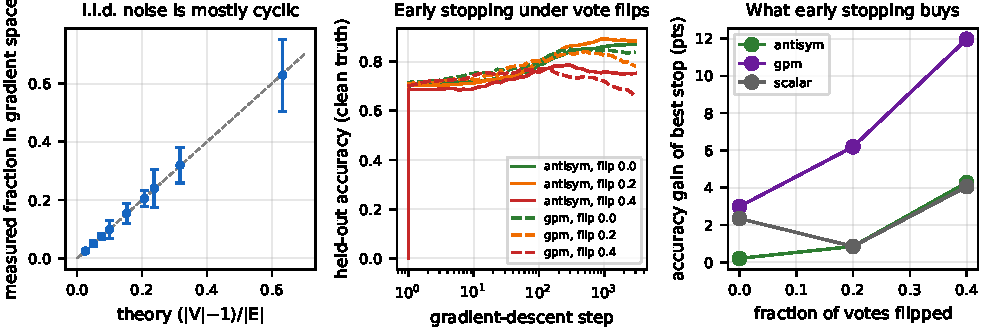
\includegraphics[width=\textwidth]{figures/noise.pdf}
\caption{Left: fraction of i.i.d.\ Gaussian edge noise in gradient space
against Lemma 2, over \NoiFracCases\ graphs (error bars: one standard
deviation over draws). Middle: held-out sign accuracy against the clean truth
during training with 0, 20 and 40\% of votes flipped (mean of seeds). Right:
accuracy gained by stopping at the best step instead of training to the end,
by model and flip rate.}
\label{fig:noise}
\end{figure*}

\paragraph{Random noise is cyclic --- annotator flips are not.} Lemma 2 holds
to within \NoiFracMaxDev\ in all \NoiFracCases\ graphs
(Figure~\ref{fig:noise}, left); on the densest graph (\NoiFracDenseN\ items,
\NoiFracDenseE\ edges) only \NoiFracDense\ of the noise is transitive. On the
synthetic task the prediction is \NoiTheoryTask\ and Gaussian noise puts
\NoiGaussGradFrac\ there. Vote flips behave differently: \NoiFlipGradFrac\ of
the resulting perturbation lies in gradient space. A flip rate $\epsilon$
pulls every win probability toward one half, so its main effect is to
\emph{shrink} the true flow --- which is mostly transitive --- rather than to
add independent noise. The clean ``noise is cyclic'' story therefore applies
to measurement noise, not to annotators who randomly disagree.

\paragraph{Early stopping helps, but not where the ranking is fitted.} Our
predicted stopping time $t^\star$, the step at which the linearised gradient
component is 95\% fitted, is too early: held-out accuracy there is
\NoiAntisymAtTstarClean\ against \NoiAntisymBestClean\ at the best step for
the antisymmetric net, because stopping when the ranking is learned also
discards the \emph{true} cycles. Early stopping still earns its keep, and more
so as noise grows (Figure~\ref{fig:noise}, middle and right). The best step
moves earlier with noise (from \NoiAntisymStepBestClean\ to
\NoiAntisymStepBestFlipFour\ steps for the antisymmetric net, \NoiGpmStepBestClean\
to \NoiGpmStepBestFlipFour\ for GPM). At 40\% flipped votes it recovers
\NoiAntisymGainFlipFour\ accuracy points for the antisymmetric net
(\NoiAntisymFinalFlipFour\ $\to$ \NoiAntisymBestFlipFour) and
\NoiGpmGainFlipFour\ for GPM (\NoiGpmFinalFlipFour\ $\to$ \NoiGpmBestFlipFour).
The scalar model, which cannot overfit cycles at all, gains
\NoiScalarGainFlipFour. The right stopping time lies \emph{between} the
gradient and cycle time scales, and where it falls depends on how much of the
cyclic content is signal. The spectrum tells us the two time scales; it cannot
by itself tell us that ratio.
